



\section{Projet de recherche: Contraindre l'origine cosmologique du champ magn\'etique cosmique avec LOFAR et NenuFAR \`a 60\,MHz}





%\section*{Le champ magn\'etique cosmologique}

\pg
Des champs magn\'etiques ont \'et\'e mesur\'es \`a presque	 toutes les \'echelles physiques de l'astronomie, allant de l'ordre du Gauss (G) sur Terre \cite{2010SSRv..152..159H}, au $\mu$G dans les galaxies \citep{2013pss5.book..641B} et amas \citep{2019SSRv..215...16V}. En-dehors des amas, le champ magn\'etique inter-galactique n'a jamais encore \'et\'e mesur\'e directement, bien que l'absence d'\'emission GeV autour de blazars d\'etect\'es en TeV \cite{2010Sci...328...73N} sugg\`ere qu'il existe. Cette contrainte observationelle sugg\`ere, de surcro\^it, que ce champ magn\'etique pourrait rester coh\'erent jusqu'\`a des \'echelles de Mpc. Son origine serait alors difficilement explicables par des m\'ecanismes astrophysiques tels que des jets \citep{2001ApJ...556..619F} ou vents galactiques \citep{2006MNRAS.370..319B}, qui op\`erent \`a plus petites \'echelles. La question est alors~: quelle est \textit{l'origine} de ce champ magn\'etique?


\begin{tcolorbox}[colback=green!10, colframe=green!50!black, arc=3mm, boxrule=1pt]
	\textbf{Probl\'ematique de recherche}~: contraindre l'origine des champs magn\'etiques inter-galactiques Mpc. 
\end{tcolorbox}

Elle ne peut pas \^etre contrainte par l'\'emission diffuse au sein des amas de galaxies, car la dynamique de formation ces structures entra\^ine de nombreux effets de saturation dynamo~: l'intensit\'e du champ magn\'etique dans les amas tend donc vers une valeur asymptote de l'ordre du $\mu$G \citep{2013A&ARv..21...62D}, ind\'ependamment de l'intensit\'e du champ magn\'etique initial. Pour contraindre l'origine du champ magn\'etique inter-galactique aux \'echelles de Mpc, il faut donc en trouver un traceur en-dehors des amas de galaxies.

\pg
L'\'evolution du champ magn\'etique dans les filaments cosmiques est domin\'ee par des m\'ecanismes de compressions et de chocs \`a petites \'echelles, capables de pr\'eserver la m\'emoire dynamique du syst\`eme, m\^eme sur des temps cosmologiques \cite{2008Sci...320..909R, 2016arXiv160207526V}, avec un champ magn\'etique d'une intensit\'e finale de l'ordre de $10^{-4} - 0.1 \mu$\,G \cite{1999A&A...348..351D, 2005ApJ...631L..21B, 2003PhRvD..68d3002S, 2008Sci...320..909R, 2009ApJ...698L..14X, 2009MNRAS.392.1008D,2015MNRAS.453.3999M}. La d\'etection de rayonnement radio-synchrotron issue de ces r\'egions permettrait alors de contraindre directement l'origine du champ magn\'etique inter-galactique \`a grande \'echelle.

\pg
Cette d\'etection est l'un des projets-cl\'es de SKA \cite{2020Galax...8...53H}, et les mod\`eles cosmologiques sugg\`erent qu'elle serait possible pour ses pr\'ecurseurs \cite{2015A&A...580A.119V} dans leurs bandes basses de $30-350$\,MHz, l'indice spectral de son \'emission radio-synchrotron serait extr\^emement pentu ($\sim -1.2 \gtrsim \alpha  \gtrsim -3$ pour $S_\nu \propto \nu^\alpha$); elle serait alors beaucoup plus forte \`a basse fr\'equence. Je propose d'anticiper SKA en d\'etectant ce signal avec LOFAR et NenuFAR.%\`A l'heure actuelle, \textit{NenuFAR est l'instrument observant aux plus basses fr\'equences accessibles depuis la Terre}. 

\begin{tcolorbox}[colback=green!10, colframe=green!50!black, arc=3mm, boxrule=1pt]
	\textbf{Projet de recherche}~: d\'etecter l'\'emission radio-synchrotron Mpc dans les filaments cosmiques \`a 60\,MHz. 
\end{tcolorbox}

\subsection{LOFAR, NenuFAR, SKA~: quelles contraintes observationelles}

\pg
La d\'etectabilit\'e de l'\'emission recherch\'ee a \'et\'e calcul\'ee pour LOFAR et SKA1-LOW \cite{2015A&A...580A.119V}. Ce calcul suppose \textit{une calibration et d\'econvolution parfaite} avec chaque instrument, ainsi que \textit{la soustraction parfaite de l'\'emission Galactique en avant-plan} \cite{2015MNRAS.447.1973B}. %La r\'ealisation de ces deux postulats est donc la premi\`ere contrainte \`a satisfaire.
Si ces contraintes sont satisfaites, alors le SKA1-LOW sera capable de d\'etecter l'\'emission recherch\'ee avec un intervalle de confiance de $3\sigma$ jusqu\`a $0.17$\,$\mu$Jy/arcsec$^2$; LOFAR-HBA jusqu'\`a $10.59$\,$\mu$Jy/arcsec$^2$; LOFAR-LBA jusqu'\`a $8.473$\,$\mu$Jy/arcsec$^2$ (voir Table 2, r\'ef.   \cite{2015A&A...580A.119V}). 
%les valeurs sont donn\'ees dans la Table 2 de \cite{2015A&A...580A.119V}. % et expliqu\'ees dans sa section 2.3.3. 
Si la magn\'etisation du milieu inter-galactique dans les filaments est de l'ordre de 1\% de l'\'energie thermique du gaz (ce gaz \'etant dans la phase Warm-Hot Interstellar Medium, ou WHIM), il \'emettra \`a un niveau de $\sim 10^{-3}-10^{-2}$\,Jy/arcsec$^2$, quelques ordres de grandeur au-dessus de la limite d\'etection de LOFAR, MWA et SKA-Low. % seront capables de d\'etecter $\sim 1\%$ de ce gas. 
A l'heure actuelle, cette \'emission n'a pas encore \'et\'e identifi\'ee~: les relev\'es LOFAR ont atteint une sensibilit\'e de $2.6$\,mJy/arcsec$^2$ \`a 144\,MHz \cite{2022A&A...659A...1S} et $382$\,mJy/arcsec$^2$ \`a 60\,MHz \cite{2023A&A...673A.165D}. LOFAR se trouve donc actuellement 10 fois au-dessus du seuil souhait\'e \`a 144\,MHz, et 50 fois \`a 60\,MHz.

\pg
La validation de l'origine de l'\'emission recherch\'ee, une fois d\'etect\'ee, se fera par deux propri\'et\'es~: son \'etendue (\'emission diffuse) et son indice spectral tr\`es pentu (compl\'etement incompatible avec l'\'emission synchrotron de galaxies radio). Il est donc critique d'am\'eliorer la sensibilit\'e de LOFAR aux basses fr\'equences. Son extension \`a Nan\c{c}ay, NenuFAR, est id\'eale pour cela. La mise en {\oe}uvre de cette am\'elioration mobilisera l'adaptation de techniques connues \`a ces pr\'ecurseurs SKA, et n\'ecessite donc une comp\'etence tr\`es sp\'ecifique. La d\'emonstration de ces techniques pemettra le futur d\'eveloppement de SKA.


\begin{tcolorbox}[colback=green!10, colframe=green!50!black, arc=3mm, boxrule=1pt]
	\textbf{Limite observationnelle}~: sensibilit\'e LOFAR \`a 60\,MHz. \textbf{Solution~:} compl\'ementer par NenuFAR. 
\end{tcolorbox}
%
%\pg
%Le rayonnement radio-synchrotron que nous souhaitons d\'etecter est tr\`es faible (champ magn\'etique faible, basse densit\'e de rayons cosmiques). Il est issu d'un plasma tr\`es diffus (opacit\'e plasma n\'egligeable). La distribution \'energ\'etique des rayons cosmiques dans ce milieu est vieille, avec un indice spectral tr\`es pentu: le rayonnement synchrotron aura donc aussi un indice spectral tr\`es pentu. Nous nous attendons donc d'avoir les meilleures chances de d\'etection aux plus basses fr\'equences radio possibles. L'ionosph\`ere de la Terre devient opaque vers $15-25$\,MHz: nous devons donc observer, id\'ealement, vers cette fr\'equence. \textbf{Seuls LOFAR et NenuFAR en sont capables} - le MWA observe jusqu'\`a 70\,MHz, et SKA-Low n'est pas encore en op\'eration.
%
%
%\pg
%De plus, nous voulons d\'etecter l'\'emission sur de larges \'echelles. Il nous faut donc un instrument sensible \`a ces \'echelles, ayant de nombreuses lignes de bases courtes. NenuFAR serait donc l'instrument parfait pour cette \'etude, avec son grand champ de vue. Cependant, il nous faut soustraire la contribution en flux provenant de sources compactes dans le champ de vue: il faut donc les r\'esoudre afin de soustraire leur contribution. LOFAR en est capable, mais souffre d'une mauvaise sensibilit\'e en-dessous de 50\,MHz.% de sa bande LBA.

\subsection{Strat\'egie~: technique et observation}

\pg
Le projet de recherche propos\'e repose sur une innovation observationnelle qui permettra de d\'epasser les limites attendues des relev\'es LOFAR, au moins \`a basses fr\'equences. Dans les ann\'ees \`a venir, le travail des relev\'es \`a 144\,MHz portera sur l'utilisation des lignes de bases internationales; avec le d\'eploiement de LOFAR2.0 pr\'evu en \'et\'e 2025, cela pourra aussi inclure leur utilisation dans les relev\'es \`a 60\,MHz. La communaut\'e s'attend donc \`a une am\'elioration d'un facteur 10 de la r\'esolution des relev\'es LOFAR existants.  

\pg
Aux plus basses fr\'equences ($30-50$\,MHz) la r\'eponse instrumentale de LOFAR est fortement d\'egrad\'ee. Cela est d\^u \`a la conception des antennes LBA, qui observent dans cette bande. Cette fen\^etre est cependant celle o\`u la chance de d\'etection du rayonnement synchrotron dans les filaments cosmiques est maximis\'ee. Les antennes de NenuFAR, bas\'ees sur le MWA, ont une r\'eponse instrumentale bien sup\'erieure aux LBA de LOFAR~: cet instrument est donc la cl\'e qui permettra d'ouvrir cette fen\^etre observationnelle. En 8 heures d'observation, le relev\'e LOFAR \`a 60\,MHz atteint une sensibilit\'e nominale de $\sim1$\,mJy; NenuFAR atteint $0.64$\,mJy avec le m\^eme temps d'int\'egration. 
L'obstacle principal, pour NenuFAR, est sa faible r\'esolution. Celle-ci entra\^ine un haut bruit de confusion \cite{1959IAUS....9..475R, 1957PCPS...53..764S} qui domine largement sur la sensibilit\'e de l'instrument. La \cref{fig.franco.sensitivity} montre les niveaux de d\'etection \`a 3$\sigma$ attendus pour LOFAR et NenuFAR \`a 50\,MHz, en utilisant la limite de confusion pour ce dernier. Le grand champ de vue permet \`a NenuFAR d'explorer efficacement les larges r\'egions o\`u le rayonnement recherch\'e pourrait se trouver. Cependant, en l'absence de d\'etection, il faudra d\'epasser le bruit de confusion. Il faut donc augmenter sa r\'esolution, en le combinant avec LOFAR.



\begin{figure}[h!]
	\centering
	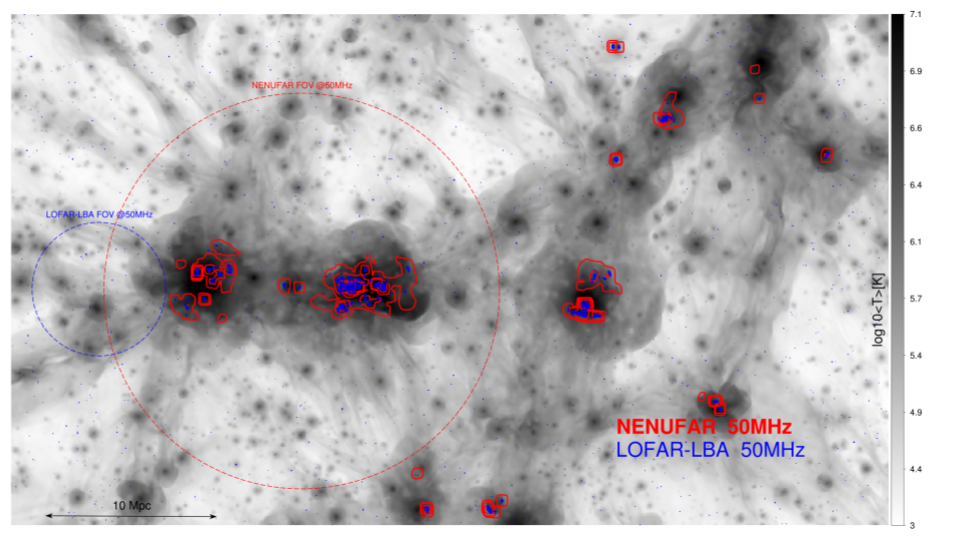
\includegraphics[width=.95\linewidth]{ProjetRecherche_futur/detection.png}
	\caption{Contours de d\'etection et champ de vue de NenuFAR et LOFAR \`a 50\,MHz. Les contours tracent la d\'etection 3$\sigma$ en l'absence d'autres sources. Figure de simulation (F. Vazza, Unibo).} \label{fig.franco.sensitivity}
\end{figure}


Mon projet de recherche se d\'eroule donc selon deux axes. D'abord, un d\'eveloppement technique et instrumental novateur, qui permettra incr\'ementalement d'atteindre de nouveaux seuils en sensibilit\'e \`a 60\,MHz. Nous y visons, chaque fois, la d\'etection du rayonnement radio-synchrotron du milieu inter-galactique dans les filaments cosmiques. Si la sensibilit\'e atteinte ne permet pas cette d\'etection, pendant le d\'eveloppement n\'ecessaire pour atteindre le prochain seuil de sensibilit\'e, nous analyserons les sources d\'etect\'ees ayant un int\'er\^et scientifique (e.g. blazars, populations de galaxies radio starburst, rayonnement fossile galactique).
La configuration observationnelle au c{\oe}ur de mon projet permettra un saut qualitatif dans la sensibilit\'e finale des relev\'es LOFAR et NenuFAR.

\newpage

\subsection{Mise en {\oe}uvre du programme de recherche}

\pg
Le c{\oe}ur de mon projet de recherche repose sur ma comp\'etence technique et instrumentale, que je propose de mobiliser pour contraindre l'origine cosmologique des champs magn\'etiques des filaments cosmiques. 
%Celle-ci me permet d'identifier de nouveaux modes d'utilisations porteurs pour les pr\'ecurseurs SKA en imagerie. Je propose de la mobiliser afin d'atteindre, incr\'ementalement, des limites de confusion plus ambitieuses, 
Il faudra, pour ce faire, atteindre des sensibillit\'es qui resteront in\'egal\'ees dans l'\`ere SKA. Je propose ainsi le plan suivant~:

\begin{tcolorbox}[colback=green!10, colframe=green!50!black, arc=3mm, boxrule=1pt]
\begin{enumerate}
	\item \textbf{2025}~: Atteindre la limite de confusion de NenuFAR (323\,mJy, r\'esolution $3'$);
	\item \textbf{2028}~: Atteindre 150\,$\mu$Jy \`a 60\,MHz (LOFAR + NenuFAR, r\'esolution $10''$);
	\item \textbf{2030}~: Atteindre 10\,$\mu$Jy \`a 60\,MHz (LOFAR-VLBI + NenuFAR, r\'esolution $1''$).
	\item \textbf{2034}~: Atteindre 20\,$\mu$Jy \`a 30\,MHz (LOFAR-VLBI + NenuFAR, r\'esolution $2''$).
\end{enumerate}
\end{tcolorbox}

%Chaque \'etape correspond \`a la limite finale possible avec les instruments utilis\'es~: la d\'epasser n\'ecessitera de nouveaux instruments. De surcro\^it, le passage d'une \'etape \`a la suivante permettra de valider des techniques et connaissances critiques pour l'exploitation optimale de SKA-Low.% Je d\'ecris le travail propos\'e pour chaque \'etape ci-dessous.


\subsubsection{Atteindre la limite de confusion de NenuFAR - amas de Coma - fin 2025}

\pg
Le projet de recherche dans son ensemble se base sur la sensibilit\'e de NenuFAR pour augmenter celle de LOFAR. La ma\^itrise technique de l'imagerie NenuFAR est donc un pr\'erequis. \`A l'heure actuelle, nous n'en sommes pas loin~: je travaille avec l'\'equipe NenuFAR pour impl\'ementer sa r\'eponse instrumentale dans des logiciels de calibration et d'imagerie qui permettront, de surcro\^it, de mitiger l'impact de l'ionosph\`ere sur la mesure. La validation de ces outils est en cours. Ils permettront \`a NenuFAR d'atteindre sa limite de confusion, de 173\,mJy \`a 66\,MHz. Cette \'etape sera la finalisation du projet pilote NenuFAR-LT09 avant le d\'eploiement d'imagerie en polarisation avec NenuFAR. %, dont les donn\'ees sont d\'ej\`a prises.

\subsubsection{Atteindre  150\,$\mu$Jy \`a 60\,MHz \`a 60\,MHz - M31 puis Coma - fin 2028}

\pg
La seconde \'etape est de combiner dans le plan Fourier des observations LOFAR et NenuFAR. Les donn\'ees LOFAR permettront de r\'esoudre les sources compactes d\'etect\'ees par NenuFAR, et donc d'en soustraire la contribution. Une technique similaire est utilis\'ee routinement avec le VLA \citep{1980ApJS...44..151T} et ses plusieurs configurations d'observation. Cette id\'ee peut sembler triviale, mais une fois valid\'ee, pourra permettre aux interf\'erom\`etres radio du futur de maximiser simultan\'ement leur r\'esolution angulaire et leur sensibilit\'e en exploitant cette option de combinaison h\'et\'erog\`ene dans leur conception. La validation s'effectuera sur un champ complexe mais bien \'etudi\'e, et susceptible d'inclure de l'\'emission compacte et diffuse~: celui de la galaxie d'Androm\`ede. Le but sera de d\'etecter l'\'emission diffuse de rayons cosmiques dans le halo de cette galaxie. Sa d\'etection imposerait de fortes contraintes sur certains mod\`eles d'auto-annihilation de mati\`ere noire \citep[e.g.][]{2016JCAP...11..021L,2022PhRvL.129k1103M}. \`A cette fin, nous avons obtenu, avec Thomas Seigert (JMU W\"urzburg) 1\,Ms d'int\'egration sur Androm\`ede avec INTEGRAL en rayons-$\gamma$ \citep{2003A&A...411L...1W}; 32h d'observations LOFAR, et 10h d'observations NenuFAR, \`a 60\,MHz. Je suis le PI de ces derni\`eres observations, qui ont \'et\'e prises \textit{dans le but} de valider la technique propos\'ee.%~: elle pourra donc \^etre effectu\'ee dans des d\'elais raisonnables.

\pg
Une fois valid\'ee, cette technique sera d\'eploy\'ee pour acc\'el\'erer d'un facteur 10.5 la recherche du le rayonnement radio-synchrotron des filaments cosmiques. Nous ferons une demande de temps d'observation NenuFAR afin de compl\'eter la couverture LOFAR du ciel Nord \`a 60\,MHz, dans le but d'atteindre la limite de confusion de LOFAR \`a 60\,MHz dans les champs extragalactiques. Nous poursuivrons ensuite cette approche sur tout le ciel Nord. % accessible \`a LOFAR et NenuFAR.

\subsubsection{Atteindre la limite de confusion de LOFAR-VLBI \`a 60\,MHz - ciel Nord - fin 2035}

\pg
La prochaine \'etape sera la r\'eduction de donn\'ees LOFAR-VLBI \`a 60\,MHz, qui est l'un des buts principaux de la collaboration Relev\'es LOFAR, et de LOFAR2.0. Ce travail se d\'eroulera sur le long terme. Ma contribution sera la prise et r\'eduction de donn\'ees NenuFAR permettant d'atteindre la limite de confusion sur tout le ciel, et le d\'eveloppement de techniques permettant le LOFAR-VLBI \`a 60\,MHz.


\subsubsection{Atteindre la limite de confusion de LOFAR-VLBI \`a 30\,MHz - ciel Nord - 2035+}

\pg
La fen\^etre de fr\'equence $30-50$\,MHz ne sera pas vis\'ee par le SKA. Ainsi, sur le long terme, LOFAR pourra basculer sur la cartographie du ciel radio \`a ces fr\'equences. Cela n\'ecessitera une am\'elioration de ses antennes LBA, et pourrait passer par le d\'eploiement de plusieurs stations NenuFAR-LSS dans le r\'eseau LOFAR. 

%
%
%\begin{tcolorbox}[colback=green!10, colframe=green!50!black, arc=3mm, boxrule=1pt]
%	
%LOFAR a pour ambition, \`a terme, de cartographier tout le ciel radio dans l'h\'emisph\`ere Nord. Le goulet d'\'etranglement pour ce projet est le champ de vue de l'ILT. Je propose de mener cette cartographie jusqu'\`a la limite de confusion de l'instrument, en commen\c{c}ant sur une surface restreinte, avec un but scientifique pr\'ecis~: contraindre une possible origine cosmologique des champs magn\'etiques pour lesquels nous d\'etecterons, dans le milieu inter-galactique des filaments cosmiques, une \'emission radio-synchrotron. 
%
%\end{tcolorbox}

\newpage

\section{Liens entre le projet et les galaxies primordiales}

\pg
Le projet d\'ecrit s'int\'eresse directement \`a des milieux inter-galactiques sur des \'echelles cosmologiques. Afin de les \'etudier, il devra atteindre des sensibilit\'es tr\`es profondes, et donc mod\'eliser et soustraire les sources ponctuelles pr\'esentes dans les champs consid\'er\'es.

\pg
Ces sources ponctuelles ont un int\'er\^et scientifique propre. G\'en\'eralement, l'\'el\'ement limitant leur \'etude est le manque de contrepartie ou d'association dans d'autres bandes. Cependant, avec les avanc\'ees actuelles du JWST, les galaxies les moins lumineuses seront d\'etect\'ees \`a la fois en infra-rouge et en radio basses-fr\'equences. La r\'esolution optique du JWST est semblable \`a celle obtenue en LOFAR-VLBI: l'association de sources d\'etect\'ees sera alors tout \`a fait naturelle. Cela permettra donc l'\'etude de larges populations de galaxies primordiales, y compris, avec LOFAR, leur budget d'\'emission d\^u \`a des processus de formation d'\'etoile en plus de leur budget d'\'emission radio provenant de noyaux actif.



\section{Insertion du projet dans le paysage SKA-LOFAR}

\pg
Mon projet de recherche s'inscrit dans les travaux de relev\'es SKA et pr\'ecurseurs. Je propose un d\'eveloppement technique qui pourrait acc\'el\'erer dramatiquement ces relev\'es, et qui serait applicable \`a de futurs t\'elescopes radios. Ce d\'eveloppement est n\'ecessaire pour la r\'ealisation de mon projet de recherche.

\pg
Ce travail se situe dans le cadre de la collaboration internationale LOFAR, avec le soutien de coll\`egues en Italie (INAF et Universit\'e de Bologne), en Allemagne (GLOW, MPFiR, TLS, et JMU W\"urzburg), au Royame-Uni (Universit\'es d'\'Edinbourg, de Durham, et de Manchester) et aux Pays-Bas (Universit\'e de Leydes). En France, il s'inscrit dans le cadre du d\'eveloppement de NenuFAR, men\'e \`a l'Observatoire de Paris, l'Universit\'e d'Orl\'eans, et l'Unit\'e Scientifique de Nan\c{c}ay.  Sorbonne Universit\'e serait donc le lieu id\'eal o\`u mener ce projet \`a bien, de par ses liens \'etroits avec ces institutions. L'\'equipe de Fran\c{c}oise Combes, au LERMA (UMR 8112), est particuli\`erement adapt\'ee \`a la mise en {\oe}uvre des premi\`eres \'etapes propos\'ees; j'y travaille d\'ej\`a avec Anne-Laure Melchior. Cela serait donc le cadre parfait pour mener la validation \`a moyen-terme de mon projet de recherche. La fusion des laboratoires actuels du LERMA, LUTH et GEPI sera le cadre id\'eal dans lequel le finaliser. Mes collaborations existantes avec le personnel de l'Observatoire et de l'USN (Philippe Zarka, Julien Girard, Alan Loh, Jean-Mathias Gri{\ss}meier, Cyril Tasse) permettra de faciliter la r\'ealisation de mon programme de recherche en prenant en compte les contraintes d'enseignement et d'organisation de la vie scientifique propres au statut de Ma\^itre de Conf\'erences.

%TODO

\section{Impact scientifique}

\pg
La d\'etection directe d'\'emission synchrotron permettra de caract\'eriser directement, pour la premi\`ere fois, les propri\'et\'es non-thermiques du milieu inter-galactique, i.e. celles de ses composantes qui ne sont pas en \'equilibre thermodynamique avec leurs environnements. Cela permettra d'\'etudier, en-dehors des amas de galaxies, les interactions entre les jets de galaxies radio et le milieu inter-galactique. 
Si la magnitude du champ magn\'etique mesur\'e dans les filaments cosmiques est compatible avec une origine cosmologique, il sera possible d'inclure de tels champs magn\'etiques dans les mod\`eles cosmologiques. 
La cartographie de la structure magn\'etique du milieu inter-galactique dans la toile cosmique ouvrira de nouveaux horizons scientifiques. Est-ce que le champ du milieu intergalactique est ordonn\'e, et jusqu'\`a quelles \'echelles? Sont-elles super-causales, et donc n\'ecessairement form\'ees plus t\^ot durant l'expansion de l'Univers? \`A quelles \'echelles commencent les champs turbulents dans le milieu inter-galactique en-dehors des amas, et \`a quels ph\'enom\`enes astrophysiques ou cosmologiques pourraient correspondre ces \'echelles?

\pg
Quant au sc\'enario n\'egatif, de non-d\'etection d'\'emission radio-synchrotron dans le milieu inter-galactique des filaments cosmiques, il permettra d'affiner la recherche avec SKA, qui a pour un de ses buts la recherche de cette \'emission. Le projet pivotera alors sur la cr\'eation d'un relev\'e profond et efficace du ciel Nord avec la technique d\'evelopp\'ee. Les relev\'es LOFAR actuels mesurent plus de 4 millions de sources avec la sensibilit\'e actuelle \cite{2022yCat..36590001S} : je propose de d\'ecupler la sensibilit\'e finale obtenue. 
Nous \'etudierons alors les propri\'et\'es des objets recens\'es, qui inclueront galaxies radio, galaxies starburst, \'emission fossile, et nouvelles d\'ecouvertes. %De surcro\^it, LOFAR \'evite jusqu'\`a pr\'esent le plan Galactique: sur le long terme, je propose de la cartographier.
%Dans une perspective technique, %ce projet l'\'emission radio-synchrotron aux plus grandes \'echelles angulaires dans la Voie Lact\'ee.


%
%\pg
%Ainsi, dans le moyen-terme, je propose d'int\'egrer mon projet de recherche dans ces efforts \`a \'echelle internationale. Le but sera de cr\'eer des relev\'es atteignant la limite de confusion de LOFAR-VLBI en LBA, sur les r\'egions autour des amas connus. Ce projet sera limit\'e par le champ de vue de LOFAR-VLBI en LBA, de l'ordre de $\sim 2 ^\circ$. Avec le b\'en\'efice de plusieurs ann\'ees dans le LERMA, j'esp\`ere aussi pouvoir commencer \`a (co)encadrer des \'etudiants de th\`ese, qui pourront b\'en\'eficier des cartes de relev\'e produites pour ce projet pour leurs \'etudes. La formation de la prochaine g\'en\'eration d'experts LOFAR-VLBI en France pourra ainsi se faire organiquement au sein du nouveau laboratoire regroupant les \'equipes du LERMA, GEPI et LUTH actuels. 

%\pg
%Dans le long terme, le projet se d\'eclinera en fonction des r\'esultats obtenus. Avec une d\'etection du signal recherch\'e, il sera possible de tenter de cartographier la toile cosmique en radio-synchrotron dans son ensemble. Cela serait un projet de tr\`es longue dur\'ee. Sans d\'etection, le programme aura alors obtenu les meilleures limites sup\'erieures \`a ce jour sur la possibilit\'e d'un champ magn\'etique d'origine cosmologique; limites qui ne seront pas d\'epassables avec d'autres instruments au sol. Notre \'equipe se tournera vers l'exploitation scientifique des informations obtenues sur les sources d'avant-plan, qui inclueront un grand nombre de galaxies radio angulairement r\'esolues \`a tr\`es basses fr\'equences.


%
%
%Je note enfin que la m\'ethode que je propose, une fois valid\'ee, pourra \^etre appliqu\'ee au reste du ciel cartographi\'e par LOFAR~: NenuFAR permettra, de par son grand champ de vue, d'obtenir tr\`es efficacement la sensibilit\'e n\'ecessaire pour atteindre le bruit de confusion de l'ILT \`a 60\'MHz, pour tout le ciel. 

%{
%\small
%\setlength{\itemsep}{0em}
%\setlength{\parskip}{0em}
%
%\bibliographystyle{aa}
%\bibliography{bib.bib}
%}


